%---------------------------------------------------------------------------------------------------------------%
\section{Fase --- B}
%---------------------------------------------------------------------------------------------------------------%


Nesta fase procedeu-se à implementação do agente e registo dos escalares
correspondentes aos parâmetros de funcionamento \texttt{R}, \texttt{D},
\texttt{N} e a chave de configuração para a operação de \emph{reset}.

Como apoio a criação de objetos da MIB, recorreu-se ao \emph{AgenPro} para gerar
uma classe com diversas classes aninhadas. Para uma melhor compreensão,
decidiu-se dividir o código nos seus diversos componentes.

Assim, na classe gerada apenas se mantêm as variáveis estáticas correspondentes
aos OID's. Como resultado, para esta fase obteve-se a classe
\texttt{ParamAuthReset} e incluiu-se numa nova, denominada
\texttt{MOScalarFactory}, alguns dos métodos da classe gerada.

Para esta fase, a classe \texttt{ParamAuthReset} manteve-se inalterada. Na
classe \texttt{MOScalarFactory}, implementaram-se 4 instancias dos objetos
escalares como \texttt{MOScalar}, todos de \texttt{Integer32}, exceto a chave de
configuração que se declarou como \texttt{OctetString}.  Dos métodos
aproveitados, temos o \texttt{createMOGroup}. Como exemplo temos o seguinte
código:


\begin{center}
\begin{minted}{java}
	//Exemplo da criação do parâmetro D
this.paramD = moFactory.createScalar(
				UminhoGrMib.oidParamD,
				moFactory.createAccess(MOAccessImpl.ACCESSIBLE_FOR_READ_ONLY), 
				(Integer32) getVariable(paramD));

	//Exemplo da criação do parâmetro da chave de configuração
this.paramAuthReset = new ParamAuthReset(
				UminhoGrMib.oidParamAuthReset,
				moFactory.createAccess(MOAccessImpl.ACCESSIBLE_FOR_WRITE), 
				agentHelper, 
				agent,
				moTableBuilder);
\end{minted}
 	\captionsetup{type=figure, width=0.8\linewidth}
	\caption{Configuração exemplo dos acessos aos objetos escalares na MIB}
\label{fig:faseb:} 
\end{center}


No código acima apenas figuram dois exemplos: para o parâmetro D e para
o parâmetro da chave da configuração (\texttt{paramAuthReset}). Para o parâmetro
D e restantes escalares foram criados com \emph{ACESSIBLE\_FOR\_READ\_ONLY}
exceto a chave. Como anteriormente foi dito, na MIB estava configurado para
\emph{read-write}, no entanto aqui, pode-se alterar para
\emph{ACESSIBLE\_FOR\_WRITE}. Além do método anterior implementou-se o interface
\texttt{MOGroup}, que permite implementar os objetos de forma atómica, aquando
o seu registo.


\texttt{Agent} é uma classe derivada de \texttt{BaseAgent}. Vários métodos foram
reescritos, porque a hierarquia assim o pede, mas alguns vazios. Por métodos que
interessam ficam o \texttt{registerManagedObject}, que recebe como parâmetro um
\texttt{MOGroup}, e o \texttt{unregisterManagedObject}. O primeiro permite
registar os objetos no servidor e o ultimo, remove os mesmos do registo. Outros
métodos importantes são o \texttt{addviews} e \texttt{addCommunities}. No
primeiro definiram-se os grupos de acesso,a s vistas e as subárvores onde se
aplicam essas permissões, ou por outras palavras se configura o VACM (\emph{View
Access Control Model}).

A \emph{Figura~\ref{fig:faseb:vacmaddgroup}} representa a primeira parte do
código do método \texttt{addviews} e, demonstra a configuração do grupo que terá
acesso à ao agente.
\begin{center}
 	 	\begin{minted}{java}

		vacm.addGroup(
			SecurityModel.SECURITY_MODEL_SNMPv2c, //Security Model
			new OctetString("c" + this.communityString), // Security Name
			new OctetString("v1v2group"), //Group Name
			StorageType.nonVolatile); // Storage type
\end{minted}
 	\captionsetup{type=figure, width=0.8\linewidth}
	\caption{Criação de grupo de acesso}
\label{fig:faseb:vacmaddgroup} 
\end{center}

A  \emph{Figura~\ref{fig:faseb:vacmaddacess}}  demonstra a configuração dos
acessos ao grupo previamente criado, onde se pode ver que não foi adicionada
qualquer verificação de identidade e foram criadas três vistas de acesso:
\texttt{fullReadView}, \texttt{fullWriteView} e \texttt{fullNotifyView}, para
leitura, escrita e notificações.
\begin{center}
 	 	\begin{minted}{java}
		vacm.addAccess(
			new OctetString("v1v2group"), //Group Name
			new OctetString(this.communityString),// Context Prefix
			SecurityModel.SECURITY_MODEL_ANY, // Security Model
			SecurityLevel.NOAUTH_NOPRIV, Security Level
			MutableVACM.VACM_MATCH_EXACT, // Match
				new OctetString("fullReadView"),  // Read View
			new OctetString("fullWriteView"),  // Write View
			new OctetString("fullNotifyView"), // Notify View
				StorageType.nonVolatile); // Storage type
\end{minted}
 	\captionsetup{type=figure, width=0.8\linewidth}
	\caption{Configuração de acessos do grupo}
\label{fig:faseb:vacmgroupacess} 
\end{center}

 A  \emph{Figura~\ref{fig:faseb:vacm}} representa a configuração para toda
 a árvore de OID's como apenas de leitura. No entanto, a configuração pode ser
 reescrita por métodos seguintes.

\begin{center}
 	 	\begin{minted}{java}
		vacm.addViewTreeFamily(
			new OctetString("fullReadView"), // View Name 
			new OID("1.3.6"), // Subtree
			new OctetString(), // Mask
				VacmMIB.vacmViewIncluded, // Type 
			StorageType.nonVolatile);// Storage type


\end{minted}
 	\captionsetup{type=figure, width=0.8\linewidth}
	\caption{Configuração das vistas de acesso para todos os objetos}
\label{fig:faseb:vacm} 
\end{center}

 A  \emph{Figura~\ref{fig:faseb:vacmtreereset}} representa a configuração da
 vista de acesso ao escalar da chave de configuração. Porém, note-se que, ao
 contrário da anterior, a vista de leitura é removida e incluída a vista de
 leitura apenas para o escalar.

\begin{center}
\begin{minted}{java}
		vacm.addViewTreeFamily(
			new OctetString("fullReadView"), // View Name 
			new OID("1.3.6.1.3.99.3.4"), // Subtree
			new OctetString(),  // Mask
				VacmMIB.vacmViewExcluded, // Type 
			StorageType.nonVolatile);  // Storage type

		vacm.addViewTreeFamily(
			new OctetString("fullWriteView"),  // View Name 
			new OID("1.3.6.1.3.99.3.4"), // Subtree
			new OctetString(),  // Mask
				VacmMIB.vacmViewIncluded, // Type 
			StorageType.nonVolatile); // Storage type

\end{minted}
 	\captionsetup{type=figure, width=0.8\linewidth}
	\caption{Configuração das vistas da subárvore da chave de configuração}
\label{fig:faseb:vacmtreereset} 
\end{center}

\newpage

 A  \emph{Figura~\ref{fig:faseb:com}} representa a implementação da configuração
 da \emph{community string}, que neste caso é lida do ficheiro de configuração.
 Note-se que se utilizou a \emph{community string} para muitos outros nomes,
 como contexto de utilização, nomes de segurança, entre outros. Poderiam ser
 outros nomes, todavia, por uma questão de homogeneidade, decidiu-se configurar
 os nomes dessa forma.
\begin{center}
\begin{minted}{java}
Variable[] com2sec = new Variable[] { 
	new OctetString(this.communityString), // community name
		new OctetString("c" + this.communityString), // security name
		getAgent().getContextEngineID(), // local engine ID
		new OctetString(this.communityString), // default context name
		new OctetString(), // transport tag
		new Integer32(StorageType.nonVolatile), // storage type
		new Integer32(RowStatus.active) // row status
};

communityMIB.getSnmpCommunityEntry().addRow(
   communityMIB.getSnmpCommunityEntry().createRow(
		new OctetString(this.communityString + "2" + this.communityString).toSubIndex(true), 
           com2sec));
\end{minted}
 	\captionsetup{type=figure, width=0.8\linewidth}
	\caption{Configuração da \emph{community string}}
\label{fig:faseb:com} 
\end{center}


Adicionalmente, criou-se uma classe denominada \texttt{AgentHelper}, cuja
instância será partilhada por outras classes. A sua implementação será
continuamente documentada durante as restantes fases deste projeto.
Nesta fase, a classe possui um metodo que lê os dados do ficheiro
de configuração e coloca em variaveis, nomeadamente porta UDP, a \emph{community
string}, o rácio de refrescamento, o tamanho da tabela e o ficheiro onde se
encontram o ficheiro com as sementes iniciais.


No método \texttt{main}, a chave de configuração é passada como argumento, bem
como a localização do ficheiro de configuração.  Em seguida é instanciada
a classe \texttt{AgentHelper}. O endereço em uso é o \texttt{0.0.0.0} e a porta
UDP é concatenada ao mesmo.  Consequentemente, a classe \texttt{Agent}
é instanciada com o endereço IP e a \emph{community string}, sendo de seguida
inicializada com o método \texttt{start}. Note-se que existem outros metodos
que não foram mencionados, mas têm a sua importância como criação de protocolos
de comunicação. O agente inicializado ativa esse protocolo, bem como aplica
a VACM configurada, entre outros.


Em seguida é criada uma instância da classe que agrupa os escalares dos
parâmetros de configuração, sendo essa instância registada no agente.  Para
manter o processo ativo deixa-se um ciclo infinito. De salientar que, em fases
seguintes existem grupos de objetos que são implementados antes dos escalares.

\subsection{Testes}

\begin{center}
 	
 	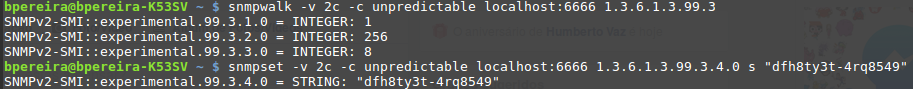
\includegraphics[width=\textwidth,height=\textheight,keepaspectratio]{resources/images/faseB/faseB.png}
 	\captionsetup{type=figure, width=0.8\linewidth}
	\caption{Testes}
\label{fig:faseB:teste} 
\end{center}






